\section{数据源与信息获取}
\subsection{领域数据源梳理}
本项目的知识来源以变构飞行器领域中文文献为主，涵盖航空航天专著、结构设计资料、飞行控制文献、气动分析文献和综述性材料。数据形态以 PDF 为主，同时存在少量扫描页、编码异常页及纯文本中间语料。项目通过 \texttt{documents.csv} 管理文档元数据，通过 \texttt{data/text\_ascii/} 与 \texttt{data/processed/sentences.jsonl} 统一管理预处理结果，从而保证后续各阶段输入的一致性和可复用性。

从来源功能上看，不同类型文献在知识图谱构建中的作用并不相同。专著适合提供较稳定的概念定义、分类体系和组成结构信息；研究论文更容易提供新方法、新参数关系和实验结论；综述文献则适合抽取领域术语、研究热点和跨文献的概念对应关系。因此，在进行数据源梳理时，项目并未将所有文献等价处理，而是从知识贡献角度理解其价值。换言之，数据源不仅是算法输入，更直接影响后续实体类型设计、关系模式覆盖范围以及图谱最终的知识密度。

从知识结构看，专著更适合提供系统性的概念层次与结构组成知识，期刊论文更适合提供参数影响、控制方法和性能分析关系，综述文献则有助于归纳领域术语体系与主要研究方向。因此，数据源梳理不仅是语料准备过程，也是后续本体设计和关系模式抽取的重要基础。

此外，原始文献在格式层面差异较大。部分 PDF 具有清晰的文本层，适合直接抽取；部分资料为扫描型页面，需要 OCR 识别；还有一些文献虽然可抽出文本，但存在严重断行、乱码、页眉页脚干扰和图表内容混入等问题。这意味着领域知识获取不能简单理解为“读取 PDF 文本”，而应被视为一项涵盖文档治理、质量控制与中间结果标准化的前处理工程。正因为本项目在数据源阶段对这些问题进行了专门设计，后续术语抽取和实体关系抽取才能获得相对稳定的输入基础。

\subsection{关键信息获取方法}
\subsubsection{面向 PDF 文献的文本提取方法}
针对中文学术 PDF 常见的编码异常、文本层混乱和扫描页问题，项目在 \texttt{preprocess/extract.py} 中设计了三级容错策略：优先使用 PyMuPDF 提取文本层；若文本质量不佳，则回退至 \texttt{pdfminer.six} 进行细粒度解析；若仍无法获得有效文本，则使用 OCR 视觉模型进行兜底识别。其核心思想是优先采用成本较低、保真度较高的抽取方式，仅在必要时升级到更强但更慢的方案。

设文档页为 \(d\)，文本质量阈值为 \(\tau\)，则可将策略抽象表示为
\[
T^*(d)=\begin{cases}T_1(d), & q_1\ge\tau \\ T_2(d), & q_1<\tau,\ q_2\ge\tau \\ T_3(d), & q_1<\tau,\ q_2<\tau\end{cases}
\]
其中 \(T_1,T_2,T_3\) 分别对应 PyMuPDF、pdfminer 和 OCR 方法，\(q_1,q_2\) 为文本质量评分。该分层处理方式兼顾了效率与鲁棒性。

为了更直观地展示文本获取和数据清洗的先后关系，图~\ref{fig:preprocess} 总结了从原始 PDF 输入到干净句子语料输出的关键处理环节。该图有助于说明本项目并不是单步抽取，而是通过多级容错和多步预处理逐渐提升文本可用性。

\begin{figure}[H]\centering
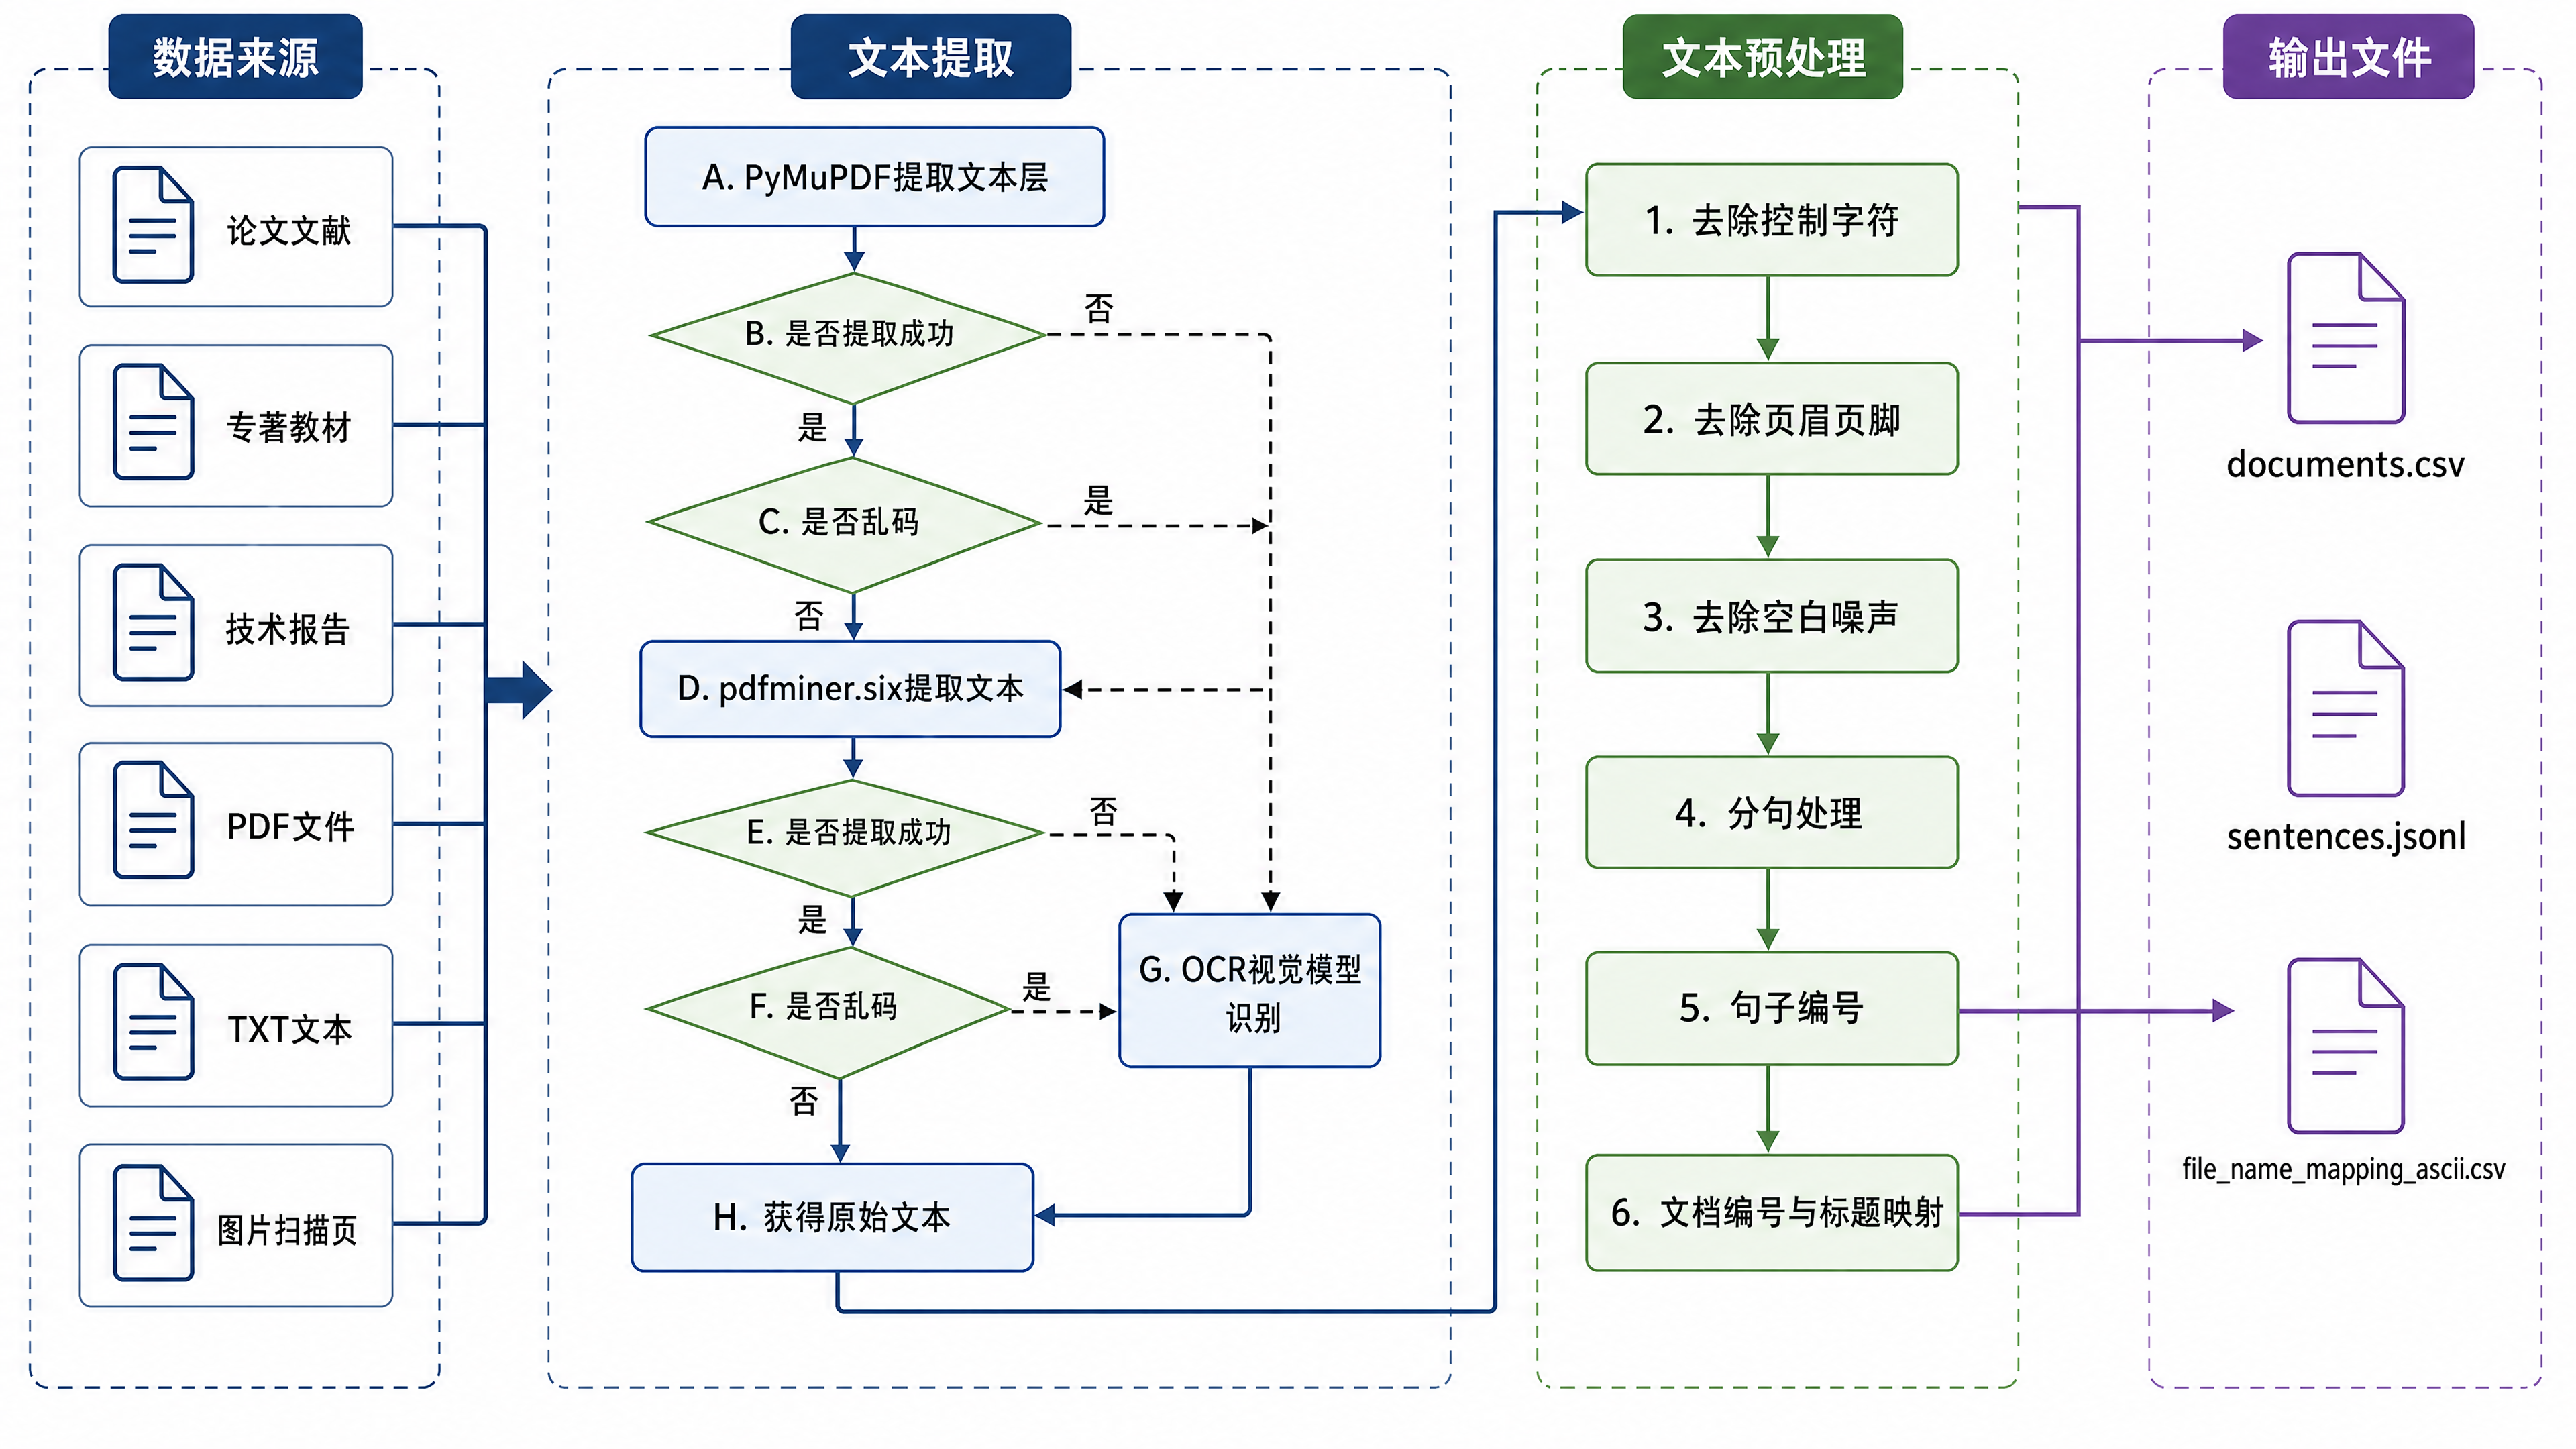
\includegraphics[width=0.88\textwidth]{figures/多源文本提取与预处理流程图.png}
\caption{多源文本提取与预处理流程图}
\label{fig:preprocess}
\end{figure}

\begin{lstlisting}[style=pythonstyle,caption={PDF 文本抽取核心策略示意}]
# preprocess/extract.py
# 1. PyMuPDF 纯文本提取
# 2. pdfminer.six 回退解析
# 3. 视觉模型 OCR 兜底
\end{lstlisting}

\subsubsection{基于术语与规则融合的数据预处理方法}
文本提取完成后，项目继续进行统一换行、去噪、分句和句子编号等处理，将原始文档转化为适合知识抽取的句子级语料。该阶段输出 \texttt{sentences.jsonl}，每条记录包含 \texttt{doc\_id}、\texttt{sentence\_id} 和文本内容，为后续术语统计和实体关系抽取提供标准输入。通过中间结果落盘，系统实现了断点续跑和阶段独立调试，体现了较好的工程规范性。

具体而言，预处理阶段不仅做了基础清洗，还重点处理了影响抽取质量的三类问题：其一是排版噪声，例如页码、重复页眉页脚和跨栏换行造成的句子断裂；其二是结构噪声，例如图题、表题、参考文献段落和公式编号混入正文；其三是语义噪声，例如长度过短且信息量不足的碎片句、过度重复的模板化句子等。通过这一系列处理，系统将面向阅读的文档格式转化为面向算法的可计算语料格式。

如果将原始文档文本序列记作 \(X=\{x_1,x_2,\ldots,x_n\}\)，则预处理函数可写为
\[
S=f_{\mathrm{clean}}(X)=\{s_1,s_2,\ldots,s_m\}
\]
其中 \(S\) 表示最终得到的句子集合。后续的术语抽取、实体识别与关系抽取均在集合 \(S\) 上进行，而不再直接依赖原始排版结构。这种“先标准化，再抽取”的策略显著提高了流水线稳定性，也便于评估阶段在句子级别进行结果对齐。

\subsubsection{利用统计方法与大模型实现关键信息抽取}
术语构建阶段是本项目的重要基础。项目在 \texttt{terminology/term\_extraction.py} 中基于 n-gram、词频、TF-IDF 与 PMI 生成候选术语，并通过综合评分进行排序。候选术语得分定义为
\[
\mathrm{Score}(t)=0.6\cdot \mathrm{freq}(t)+0.3\cdot \mathrm{tfidf}(t)+0.1\cdot \max(\mathrm{PMI}(t),0)
\]
其中 \(t\) 为候选术语，词频体现语料覆盖度，TF-IDF 体现区分能力，PMI 体现术语内部搭配紧密度。该阶段以较高召回率保留潜在领域词，然后通过大模型完成术语是否保留、规范名称和实体类型的定稿判断。这种“先统计、后语义精筛”的方式是本项目的重要创新点之一。

为了增强系统的领域泛化能力，我们对大模型的系统 Prompt 进行了拓展，将其适用范围从单一的“航空航天”扩展至“通用机械与工程（含汽车、液压等）”领域，有效避免了非航天专业文献中通用工程术语被错误过滤的问题。此外，系统还实现了基于 LLM 的增量词典融合与审核机制：在多文档并发上传的场景下，系统会自动读取已有的术语金标准，并与新文档抽取的术语进行去重与融合，从根本上解决了多次上传导致旧图谱内容被覆盖的增量构建难题。

\begin{lstlisting}[style=pythonstyle,caption={候选术语生成示意}]
def generate_candidate_terms(tokens, max_ngram=4):
    counter = Counter()
    ...
    return counter
\end{lstlisting}

\subsection{基于规则约束的知识抽取方法}
在获得术语表后，系统进入实体识别与关系抽取阶段。实体识别采用词典最长匹配和规则补充相结合的方法；关系抽取则采用双模混合逻辑：在有标准词典的明确语境下，结合触发词、位置约束、实体距离阈值和类型约束生成三元组以保证极高的可解释性；而在长难句或隐式关联场景下，系统会自动无缝切换至 LLM 抽取模式进行知识拓扑补全。与完全开放的单一黑盒抽取方式相比，本项目的双模设计更加注重结果质量、可解释性和图谱可展示性。
